\chapter{Introduzione}
\label{cha:intro}


La presente tesi è il risultato del tirocinio curriculare che ho svolto negli scorsi mesi, nell'ambito del progetto Community Health Metrics di Wikipedia.
Tale iniziativa ha l’obiettivo di misurare lo stato di salute delle comunità di Wikipedia attraverso 6 metriche,
fornendo strumenti utili per analizzare la partecipazione degli editor e supportarne lo sviluppo nel tempo.

Il punto di partenza del mio lavoro era costituito da uno script monolitico che,
pur permettendo di calcolare le metriche desiderate, presentava diversi limiti in termini di modularità,
scalabilità e assenza di strumenti di monitoraggio.

L’attività di tirocinio si è quindi focalizzata sul refactoring di questo sistema,
con l’obiettivo di realizzare una pipeline dati moderna e automatizzata, basata su Apache Airflow, e integrata con un sistema di monitoraggio fondato su Prometheus e Grafana.
Il lavoro si è infine concluso con il deploy in produzione della pipeline su un server Wikimedia,
dove è attualmente utilizzata per il calcolo mensile delle metriche.

\section{Contesto}
\label{sec:contesto}
Il progetto Community Health Metrics propone sei insiemi di indicatori, detti Vital Signs, per valutare crescita e rinnovamento delle comunità di Wikipedia.
Tre riguardano l’intera popolazione di active editors (chi crea contenuti):
Retention, Stability e Balance;
tre riguardano funzioni comunitarie specifiche: Special functions, Administrators e Global participation.

Di seguito presento in dettaglio come vengono misurati questi indicatori e quali sono le metriche associate:

\begin{itemize}
    \item \textbf{Retention}: Misura la capacità di trattenere i nuovi editori nel tempo. L’indicatore base è la retention rate: quota di nuovi editori che effettuano almeno un’altra modifica 60 giorni dopo la prima. È un segnale precoce della qualità dell’onboarding e dell’inclusione dei newcomer.
    \item \textbf{Stability}: Cattura la persistenza degli editori attivi. Si conta il numero di mesi consecutivi di attività per ogni editor e si analizza la distribuzione in sei fasce: 1 mese, 2 mesi di fila, 3-6, 7-12, 13-24, più di 24 mesi. Una comunità “stabile” combina sia nuove presenze sia contributori di lungo periodo.
    \item \textbf{Balance}: Valuta l’equilibrio tra “generazioni” di editor molto attivi. L’indicatore considera numero e percentuale di very active editors per anno e per generazione (definita come il lustrum dell’anno del primo edit). Un editor "very active" è un utente registrato (non bot) con più di 100 edit al mese nel mainspace. L’obiettivo è che più generazioni contribuiscano alla “spina dorsale” produttiva, senza dipendere solo dai veterani.
    \item \textbf{Special functions}: Questo indicatore prende in considerazione gli editor che svolgono compiti speciali all’interno di Wikipedia, ossia attività che vanno oltre la semplice scrittura di contenuti. In particolare, vengono distinte due categorie: da un lato coloro che si occupano della manutenzione tecnica, contribuendo nei namespace relativi a template e infrastruttura del software; dall’altro chi partecipa alle attività di coordinamento, interagendo negli spazi dedicati all’organizzazione e alla governance della comunità.
    \item \textbf{Administrators}: Gli amministratori svolgono un ruolo centrale nel mantenimento dell’ordine e della qualità all’interno delle comunità di Wikipedia, poiché hanno la responsabilità di supervisionare i contenuti, applicare le regole e garantire il corretto funzionamento del progetto. Per valutare la capacità di questo gruppo di supportare la comunità, l’indicatore osserva sia l’evoluzione storica degli utenti che hanno ricevuto i permessi amministrativi, sia il numero di amministratori effettivamente attivi nel tempo. Un altro aspetto rilevante riguarda il rapporto tra amministratori ed editor attivi: questo valore fornisce un’indicazione della sostenibilità del gruppo di gestione rispetto alla dimensione complessiva della comunità. In questo modo è possibile comprendere se il numero di amministratori è sufficiente a garantire trasparenza ed efficienza, evitando situazioni di sovraccarico o, al contrario, un eccesso di concentrazione di potere decisionale.
    \item \textbf{Global participation}: Questa metrica misura il grado di apertura e di interconnessione di una comunità linguistica di Wikipedia con il resto del movimento Wikimedia. Da un lato considera il livello di partecipazione degli utenti al progetto Metawiki, osservando in particolare quanti editor attivi hanno come lingua primaria quella della comunità analizzata. Dall’altro analizza la composizione degli editor in base alla loro lingua primaria, distinguendo tra chi contribuisce principalmente nella Wikipedia in questione e chi invece proviene da altre edizioni linguistiche. In questo modo è possibile valutare la capacità della comunità di attrarre contributori multilingue e di favorire interazioni tra diverse wiki, elementi importanti per garantire apertura, collaborazione e scambio con il resto dell’ecosistema Wikimedia.
\end{itemize}

Le metriche descritte vengono calcolate a partire dai MediaWiki History Dumps, un insieme di file che documentano in maniera completa la cronologia delle modifiche di Wikipedia e che vengono aggiornati mensilmente. Questi dataset rappresentano la base informativa su cui si fonda il progetto Community Health Metrics, in quanto permettono di ricostruire l’evoluzione delle comunità e di derivarne gli indicatori presentati. Nel capitolo successivo verranno presentati nel dettaglio la loro struttura e i dataset utilizzati nella fase di sviluppo della pipeline.
\section{Dataset}
\label{sec:dataset}
Il dataset dei MediaWiki History Dumps contiene la cronologia completa degli eventi relativi a revisioni, utenti e pagine delle wiki Wikimedia a partire dal 2001. I dati sono organizzati in uno schema denormalizzato, in cui tutte le informazioni sono raccolte in un unico formato, includendo campi precomputati utili alle analisi, come il numero di edit per utente e per pagina o le operazioni di revert. Questo rende i dumps una fonte strutturata e coerente per lo studio dell’evoluzione delle comunità.
Il dataset dei MediaWiki History Dumps viene aggiornato con cadenza mensile, generalmente entro la fine della prima settimana del mese. Ogni rilascio contiene l’intera cronologia a partire dal 2001 fino al mese corrente: questo approccio è necessario poiché eventi come rinomini di utenti, revert o spostamenti di pagine possono modificare retroattivamente lo stato delle tabelle, rendendo poco affidabili eventuali aggiornamenti incrementali.
I dumps sono organizzati secondo un sistema di partizionamento che tiene conto della dimensione delle diverse edizioni linguistiche. Per le wiki più grandi, come enwiki, wikidatawiki e commonswiki, i file sono suddivisi su base mensile; per quelle di dimensioni intermedie la suddivisione è annuale; mentre per le comunità più piccole l’intero storico è raccolto in un singolo file. In questo modo si evita la generazione di file eccessivamente voluminosi, mantenendo ogni dump entro la dimensione di circa 2 GB.
I dumps sono distribuiti in formato TSV, compresso con Bzip2 per ridurre le dimensioni.
La struttura delle directory segue una convenzione che comprende la versione del dump (nel formato YYYY-MM, con la disponibilità limitata agli ultimi due mesi), il nome della wiki e l’intervallo temporale della partizione, ad esempio: /2019-12/ptwiki/2019-12.ptwiki.2018.tsv.bz2.

Nel contesto del progetto ci interessano esclusivamente i dumps relativi alle comunità linguistiche di Wikipedia, poiché costituiscono la base per il calcolo delle metriche presentate. Nella fase di sviluppo ho scelto di lavorare su un sottoinsieme di questi dati, selezionando alcune edizioni linguistiche dei dialetti italiani: piemontese, lombardo, ligure, veneto, sardo, siciliano e napoletano. La scelta è stata guidata dal fatto che tali dataset, oltre ad avere dimensioni ridotte, sono distribuiti in un unico file all-time, caratteristica che li rende particolarmente adatti per le fasi di test e sviluppo.

Per chiarezza, nella tabella seguente riporto le edizioni considerate, con il nome della lingua, il codice corrispondente e la dimensione del file dump in megabyte:
\begin{table}[htbp]
    \centering
    \begin{tabular}{|l|c|c|}
        \hline
        \textbf{Lingua} & \textbf{Codice} & \textbf{Dimensione (MB)} \\
        \hline
        Piemontese & pmswiki & 64.6 \\
        Lombardo   & lmowiki & 91.6 \\
        Ligure     & lijwiki & 18.9 \\
        Veneto     & vecwiki & 78.9 \\
        Napoletano & napwiki & 45.3 \\
        Siciliano  & scnwiki & 57.4 \\
        Sardo      & scwiki  & 14.6 \\
        \hline
    \end{tabular}
    \caption{Dump utilizzati nella fase di sviluppo (edizione maggio 2025)}
    \label{tab:dumps_sviluppo}
\end{table}


\section{Problema affrontato}
\label{sec:problema_affrontato}

La versione iniziale dell’architettura, disponibile su GitHub, era costituita da un unico script Python, denominato vital\_signs.py. Questo programma aveva il compito di estrarre i dati dai MediaWiki History Dumps e di popolare due database SQLite. Le operazioni venivano eseguite in maniera sequenziale: in una prima fase lo script generava il database vital\_signs\_editors.db, contenente le informazioni di base sugli editor. Successivamente, a partire da questi dati, calcolava gli indicatori definiti come Vital Signs e li inseriva nel database vital\_signs\_web.db.


Quest’ultimo database rappresentava l’output finale del processo ed era utilizzato da un’applicazione sviluppata con il framework Dash, che permetteva di visualizzare graficamente gli indicatori attraverso una serie di dashboard.
Questa applicazione è stata sviluppata da un altro tirocinante ed era stata deployata su un server wikimedia dedicato, dove era accessibile pubblicamente.

\begin{figure}[htbp]
    \centering
    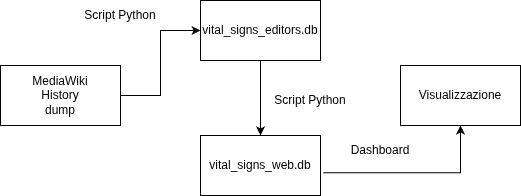
\includegraphics[width=\linewidth]{img/oldarch.png}
    \caption{Rappresentazione logica della vecchia architettura}
    \label{fig:oldarch}
\end{figure}
L'architettura presentava diversi limiti:
\begin{itemize}
    \item \textbf{Monoliticità}: Tutte le operazioni erano contenute in un unico script, rendendo difficile la manutenzione e l'estensione del codice. Non c'era modularità, né possibilità di riutilizzare le singole parti del processo.
    \item \textbf{Assenza di schedulazione}: Lo script doveva essere eseguito manualmente, senza alcun meccanismo di schedulazione. Questo rendeva impossibile automatizzare l'aggiornamento dei dati, che doveva essere fatto manualmente ogni mese.
    \item \textbf{Mancanza di monitoraggio}: Non c'erano strumenti per monitorare lo stato di esecuzione dello script, né per raccogliere metriche sulle performance. In caso di errori, non era possibile risalire facilmente alla causa.
    \item \textbf{Prestazioni limitate}: L'approccio sequenziale e la mancanza di parallelizzazione rendevano il processo lento, soprattutto con dataset di grandi dimensioni. Non c'era modo di scalare l'elaborazione per gestire volumi crescenti di dati.
    \item \textbf{Difficoltà di deploy}: trattandosi di uno script, il deploy risulta più complicato rispetto ad un approccio basato su container. Non c'era isolamento tra le dipendenze e l'ambiente di esecuzione, rendendo difficile la gestione delle versioni e delle librerie.
\end{itemize}

\subsection{Obiettivi del tirocinio}
\label{subsec:obiettivi_tirocinio}

L’obiettivo principale del tirocinio è stato il refactoring dello script esistente e la progettazione di una data pipeline completamente automatizzata utilizzando Apache Airflow. In particolare, il lavoro ha previsto:

\begin{itemize}
\item la strutturazione del workflow in task modulari e indipendenti, per garantire chiarezza e riusabilità;
\item l’introduzione di meccanismi di schedulazione, così da consentire esecuzioni periodiche e affidabili senza intervento manuale;
\item l’integrazione di strumenti di monitoraggio per tracciare lo stato della pipeline e raccogliere metriche di performance;
\item lo sviluppo dell’intera infrastruttura in un ambiente Docker, con tutti i componenti (Airflow, database e monitoring stack) containerizzati e orchestrati tramite docker-compose, al fine di semplificare il deploy e garantire portabilità;
\item la sostituzione del database SQLite con PostgreSQL, scelta resa necessaria dal fatto che le task in Airflow vengono eseguite in parallelo e quindi richiedono un sistema in grado di gestire operazioni concorrenti in scrittura;
\item il deployment della nuova architettura su un server Wikimedia, dove la pipeline è ora attiva in produzione e calcola mensilmente le metriche richieste.
\end{itemize}

Nei capitoli successivi vengono presentate in dettaglio le tecnologie utilizzate (Capitolo~\ref{cha:tecnologieutilizzate}), l’implementazione della nuova architettura (Capitolo~\ref{cha:implementazione}), e infine i risultati ottenuti e le conclusioni del lavoro (Capitolo~\ref{cha:risultaticonclusioni}).

\clearpage